\documentclass{article}


\usepackage{PRIMEarxiv}
\usepackage{amsmath}

\usepackage{amssymb}
\usepackage{amsfonts}
\usepackage{algorithm}
\usepackage{algpseudocode}

\usepackage[utf8]{inputenc} % allow utf-8 input
\usepackage[T1]{fontenc}    % use 8-bit T1 fonts
\usepackage{hyperref}       % hyperlinks
\usepackage{url}            % simple URL typesetting
\usepackage{booktabs}       % professional-quality tables
\usepackage{amsfonts}       % blackboard math symbols
\usepackage{nicefrac}       % compact symbols for 1/2, etc.
\usepackage{microtype}      % microtypography
\usepackage{lipsum}
\usepackage{graphicx}
\graphicspath{{IMGS/}}     % organize your images and other figures under media/ folder

  
%% Title
\title{RL: Learn to Cut Project Report
}

\author{
  Leon Li \\
  Columbia University \\
  Computer Science Department\\
  \texttt{\{al4263\}@columbia.edu} \\
}


\begin{document}
\maketitle


\begin{abstract}
Integer programming, in theory, is an NP-hard problem. In the paper Reinforcement Learning for Integer Programming: Learning to Cut \cite{rlcut}, the author used a RL approach to solve the problem that significantly outperforms human-designed heuristics. In this report, we followed the work done by the authors, with some innovations and adaptations, to tackle IP. The adapted methods can (1) tackle even more difficult IP problems and (2) generalize to new instances.
\end{abstract}





\section{Introduction and problems}
The problem set up is the following:

\[  \min \{c^Tx : Ax \leq b,x\geq0, x\in \mathbb{Z}^n \} \]
The Gomory cuts provide an effective method to solve integer programming. At each iteration, the Gomory cuts algorithm provides a set of possible cuts for us to cut the plane, which is adding more constraints. The goal is to find the optimality gap by adding more cuts, which is to optimize $OPT_{LP} - OPT_{Integer}$ \cite{lecture} by adding more constraints to the integer programming.

Here, we can formulate the problem in the RL diagram: 
Let $n$ be the number of variables:

At the $t = 0$, the state space is the set of all constraint: \textbf{S} = $\{A_t x \leq b_t \}$ where $\forall a_i \in A_t, a_i \in \mathbb{R}^n$ and  $\forall b_i \in b_t, b_i \in \mathbb{R}$.

The action space is the possible new constraints/cuts generated by the Gomory cuts: \textbf{A} =  $\{E_t x \leq d_t \}$ where $\forall e_i \in E_t, e_i \in \mathbb{R}^n$ and  $\forall d_i \in d_t, d_i \in \mathbb{R}$.

The transition from $s_t$ to $s_{t+1}$ is simply adding the cut into the previous state as a new constraint.

Let $x^*_{LP}$ be the optimal solution, the reward is $C^T x^*_{LP}(t+1) - C^T x^*_{LP}(t) \geq 0.$ We also use discounted reward with $\gamma$ to encourage the agent to find the solution early.


\section{Algorithm and Training method}
\subsection{Policy Architecture: LSTM and Attention}

The policy $\pi$ samples an action from the action space each time: $a = \pi(s_t ; \theta)$. The policy is a parametrized neural network.The core dilemma is that size of state and action space is not fixed. To solve this problem, we use the LSTM\cite{lstm} and the Attention Mechanism\cite{attention1}\cite{attention2}. First of all, we concatenate $A$ and $b$ and call it the constraint matrix, and concatenate $E$ and $d$ call it the candidate matrix. At time step $T = t$, the constraint matrix is a matrix with the shape of $\mathbb{R} ^ {(m+t) \times (n+1)}$, where $m+t$ is the number of constraints and $n$ is the number of variables. Similarly, for the candidate matrix, it is a matrix with the shape of $\mathbb{R} ^ {(k) \times (n+1)}$, where $k$ is the number of candidate Gomory cuts. The core idea of the algorithm is to calculate the attention score for each cuts in the candidate with all the constraint in the constraint matrix.\cite{rlcut} And the candidate with the highest attention score will be the most aligned with the set of constraints, which means the cuts with the highest reward. 

The implementation is the following: we first use an LSTM with hidden dimension of $32$ to embed the constraint matrix and candidate matrix. Here, we use the last hidden cell output of the LSTM as the final embedding. For the embedding, we pass it to a 2 hidden layer neural network with hidden unit of size $64$ and Tanh nonlinear activation functions. The output dimension is $k = 16$. Let's call the embedded constraint matrix as $H$ and the embedded candidate matrix as $G$. The attention score matrix is calculated as
 \[S_j = \frac{1}{N_t}\sum_{i=1}^{N_t} g_j^Th_i \text{$\forall$ $h_i$, $g_j$ in H, G} \]
 
 The action is then simply the argmax over the Softmax of the attention score.

\subsection{Policy Training: Policy Gradient}

The policy gradient is: 

$$\nabla_\phi \rho(\phi) = \mathbb{E}_{\pi} \big[\sum_{t=0}^\infty Q^{\pi_\theta}(s_t,a_t) \nabla_\theta \log \pi(s_t, a_t ; \theta) \big]\cite{pg}$$
To compute the gradient and update $\theta \leftarrow \theta + \alpha \nabla_\theta \rho(\theta)$, where $\alpha$ is the learning rate, we need to find the value of
 $Q^{\pi_\theta}(s_t,a_t)$. However, it is not analytically solvable, and thus requires us to estimate with either Monte Carlo estimation, or train a Value function as the baseline( Actor-Critic). In this problem, we simply sample one trajectory of cuts, which is one episode with discounted reward with $\gamma$, and compute the loss and gradient estimator $\hat g$ as the following: 

For one trajectory of collected estimated $Q_s$ and a list of state action pairs $(s(t = i), a(t = i))$, the Loss is defined as $-\frac{1}{N} \sum_{i=1}^N Q_s(t = i) \log(\pi(s(t = i), a(t = i) ; \theta)) $, and the gradient estimator $\hat g$ is:

$$- \frac{1}{N} \sum_{i=1}^N Q_s(t = i)  \nabla_\theta \log(\pi(s(t = i), a(t = i) ; \theta)\cite{pg} $$

\subsection{Evolution Strategies}
For the evolution strategies, I did not strictly follow what was described in the paper \cite{rlcut}. The core idea of es is to calculate the noisy estimation of the performance of policy $\pi_\theta$. Thus we use the following noisy estimation of the $Q$ generated by policy $\pi_\theta$:

$$Q_i \leftarrow Q_i + \alpha \epsilon_i \text{, where } \alpha = 0.15 \text{ and } \epsilon_i \sim \mathcal{N}(0,1)$$

\subsection{Curriculum Training}

The easy configuration has 10 instances, where the hard configuration has 100 instances. To directly train the policy network on the hard configuration is extremely challenging. Instead, we propose the method of curriculum training: we generate three curriculums consists of 10, 40, 70 instances separately, and we train the same policy network on those three curriculum dataset first, and then train it on the hard configuration.

\subsection{Data Processing}

Data processing is extremely useful for deep learning tasks. In this task, we want to process both the constraint matrix and the candidate matrix. However, we do not want to lose the relative information about the constraint and the candidate, as numerical relationships are extremely useful. So we concatenate both the constraint and candidate matrix together and then standardize the matrix by subtract the mean and then divide the variance.


\subsection{Pseudo code}


Here are the algorithm for both easy config training and hard config training. Some terminology: $L_C, L_D, L_A, L_R$ refers to the list to record the constraint, candidates, actions, and rewards. $E_r$ refers to the cumulative episode rewards without discounting. $ND$ refers to not done, which is the condition that $x^*_{LP}(t)$ is not all integer value. $C$ is the state, which is the constraint matrix, and $D$ is the candidate space.

\begin{algorithm}[H]
\caption{Training \cite{rlcut}}\label{alg:cap}
\begin{algorithmic}[1]
\State Input: initialize a policy $\pi_\theta$, IP instance parameterized by c, A, b, timelimits T 
\State Hyperparameter: learning rate $\alpha$, ES random rate $\sigma$
\For{$e_t \in$ episodes} 
\State reset environment, initialize t = 0, $E_r$ = 0, empty lists to record $L_C, L_D, L_A, L_R$
\State $C(0) = [A,b]$, find $x^*_{LP}(0)$ and $D(0) = [E,d]$
\While{ND and t < T}
	\State $s_t = \{C(t), D(t), x^*_{LP}(t)\}$
	\State standardize $C(t)$ and $D(t)$
	\State compute attention score with $att_{score}(t) = \pi_\theta(C(t), D(t))$
	\State sample action as $a(t)$ = argmax of softmax($att_{score}(t)$) 
	\State find the reward $r(t)$
	\State generate $C(t+1)$ by append the cut to $C(t)$
	\State append $C(t), D(t), a(t), r(t)$ to  $L_C, L_D, L_A, L_R$
	\State $E_r \gets E_r + r(t)$
	\State $t \gets t + 1$
\EndWhile
\State calculate discounted reward $d_r$
\State calculate $Q_s$ with $d_r$ and ES
\State use  $L_C, L_D, L_A, L_R, Q_s$ to compute the gradient estimator $\hat g$
\State $\theta \gets \theta + \alpha \hat g$
\EndFor \\
\Return $\theta$
\end{algorithmic}
\end{algorithm}

The algorithm for curriculum training is:
\begin{algorithm}[H]
\caption{Curriclum Traning}\label{alg:cap}
\begin{algorithmic}[1]
\State Input: initialize a policy $\pi_\theta$, Curriclums, hard config 
\For{curriculum$(i)$ $\in$ Curriclums} 
\State Train the network $\pi_\theta$ with the Training algorithm above
\EndFor
\State Train the network $\pi_\theta$ with hard config \\
\Return $\theta$
\end{algorithmic}
\end{algorithm}

The roll out of the policy:
\begin{algorithm}[H]
\caption{Roll out of policy}\label{alg:cap}
\begin{algorithmic}[1]
\State Input: a trained policy $\pi_\theta$, IP instance parameterized by c, A, b, time limits T
\State reset environment, initialize t = 0, $E_r$ = 0
\State $C(0) = [A,b]$, find $x^*_{LP}(0)$ and $D(0) = [E,d]$
\While{ND and t < T}
	\State $s_t = \{C(t), D(t), x^*_{LP}(t)\}$
	\State standardize $C(t)$ and $D(t)$
	\State compute attention score with $att_{score}(t) = \pi_\theta(C(t), D(t))$
	\State sample action as $a(t)$ = argmax of softmax($att_{score}(t)$) 
	\State find the reward $r(t)$
	\State generate $C(t+1)$ by append the cut to $C(t)$
	\State $E_r \gets E_r + r(t)$
	\State $t \gets t + 1$
\EndWhile \\
\Return $E_r$

\end{algorithmic}
\end{algorithm}


\section{Result}
\subsection{easy configuration}
Here is the result for easy configuration: 
\begin{figure}[h]
\centering
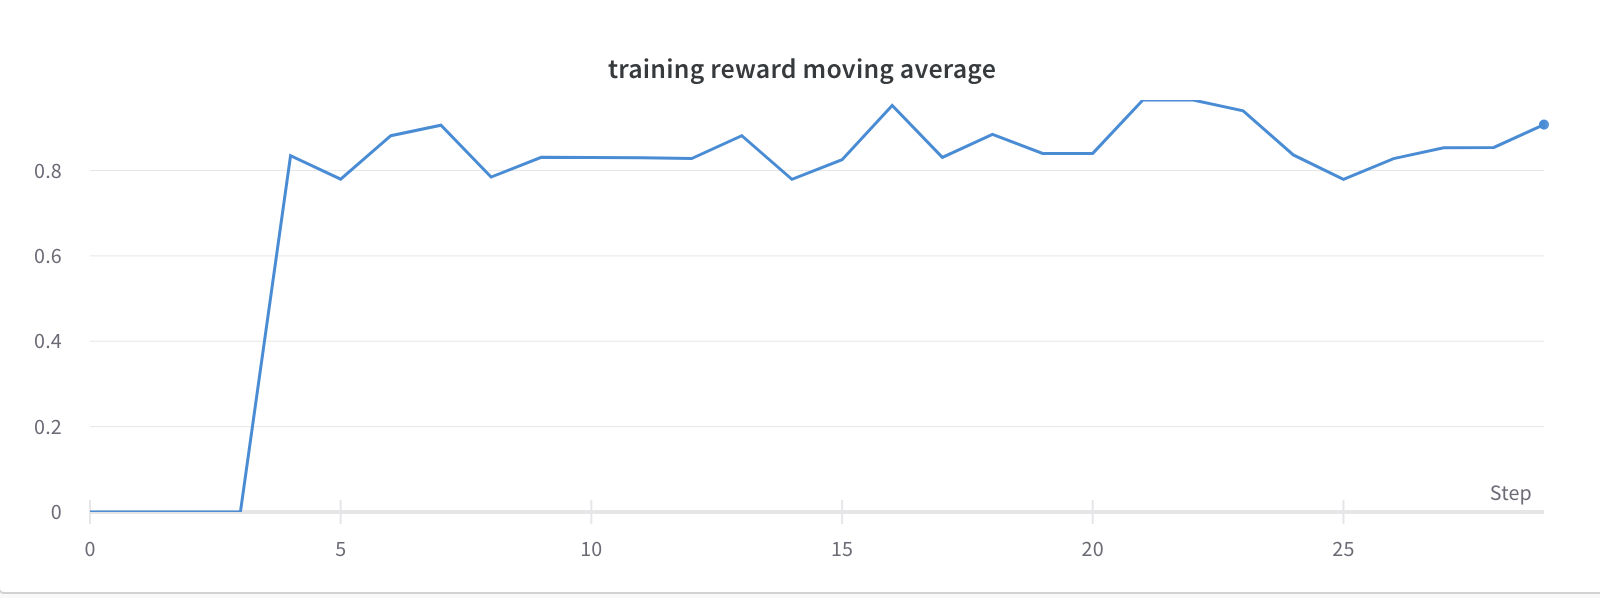
\includegraphics[width=1\textwidth]{easy_config.png}
\caption{Averaged Moving Reward within 10 steps for easy configuration}    
\end{figure} 

\subsection{hard configuration}
Here is the result for easy configuration: 
\begin{figure}[h]
\centering
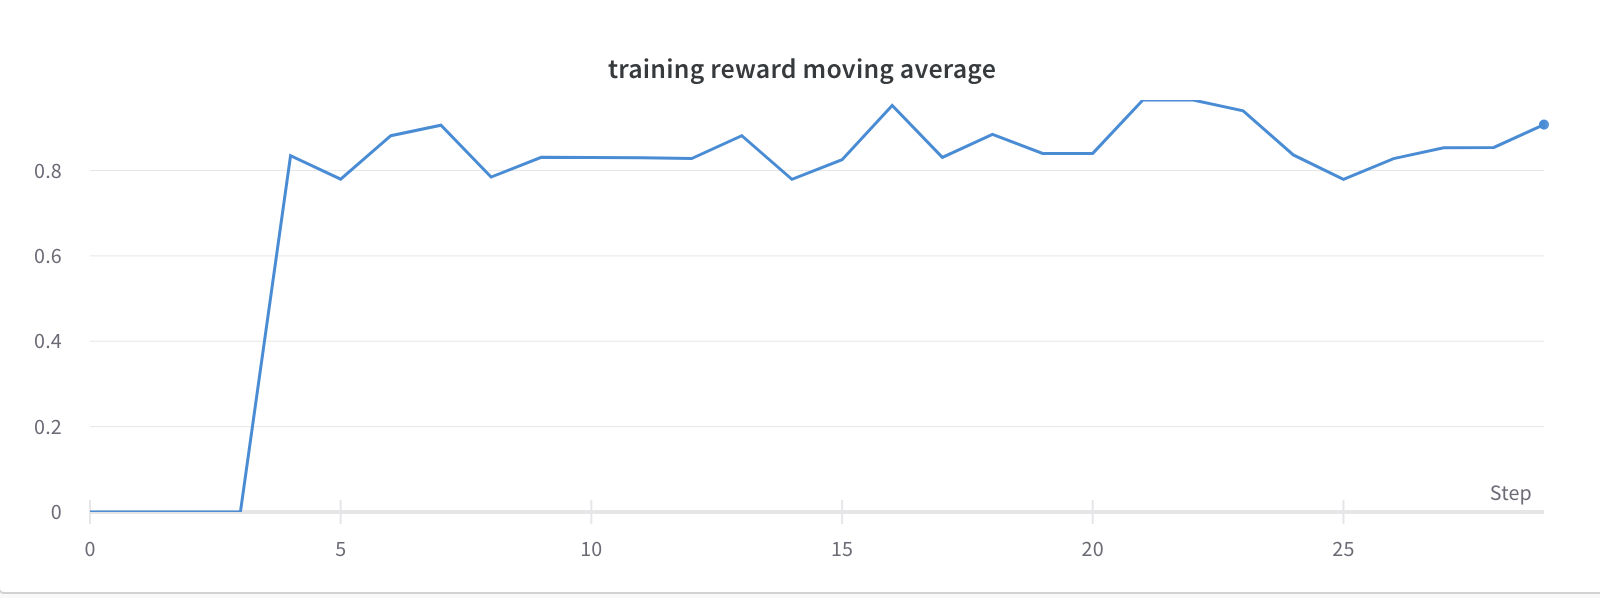
\includegraphics[width=1\textwidth]{easy_config.png}
\caption{Averaged Moving Reward within 10 steps for easy configuration}    
\end{figure} 


\subsection{test configuration}
Here is the result for easy configuration: 
\begin{figure}[h]
\centering
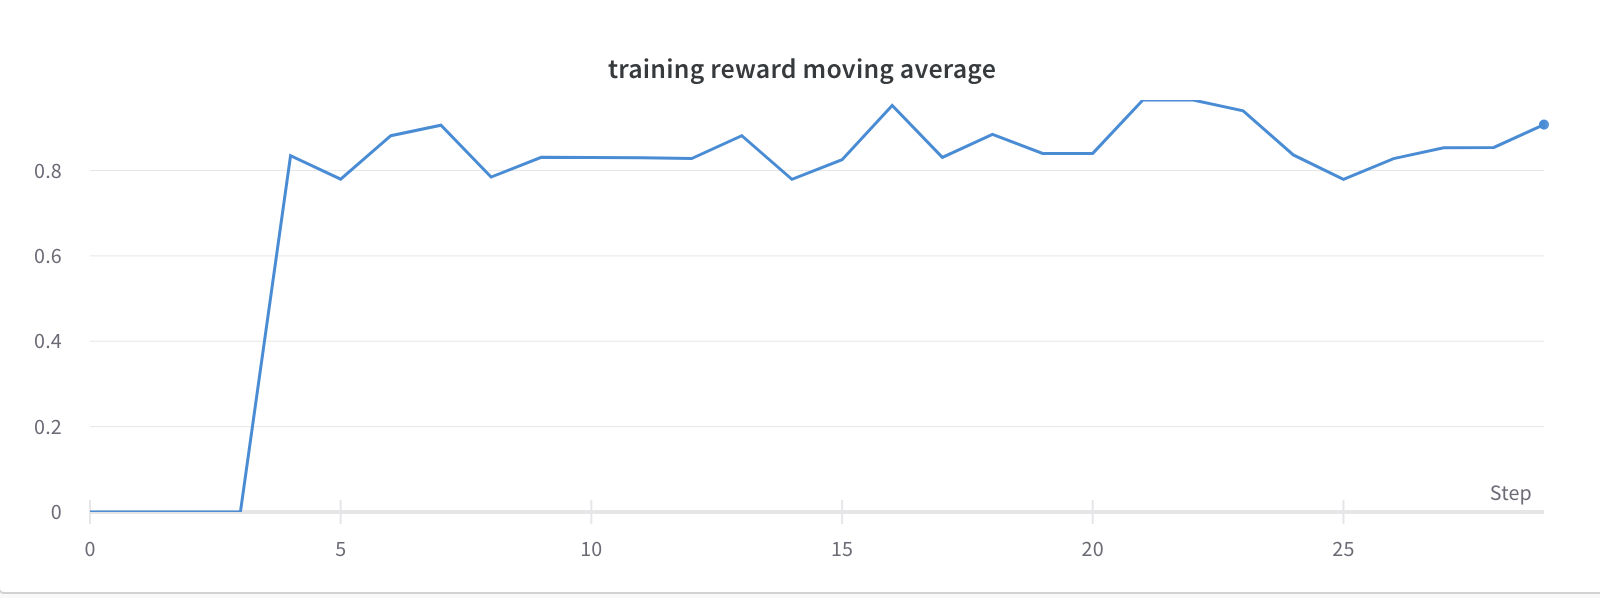
\includegraphics[width=1\textwidth]{easy_config.png}
\caption{Averaged Moving Reward within 10 steps for easy configuration}    
\end{figure} 



%Bibliography
\bibliographystyle{unsrt}  
\bibliography{references}  


\end{document}
